\documentclass[12pt]{article}
\usepackage[margin=1in]{geometry}
\setlength{\parindent}{0pt}
\setlength{\parskip}{5pt}
%\pagenumbering{gobble}% 

\usepackage{amsmath,amsthm,amssymb}
\usepackage{graphicx}
\usepackage{bm}
\usepackage{float}
\newtheorem{euclidtheorem}{Proposition}[section]
\newtheorem{classtheorem}{Theorem}
\newtheorem{theorem}{Theorem}[section]
\newtheorem{challenge}[theorem]{Challenge}
\newtheorem{question}[theorem]{Question}
\newtheorem{problem}[theorem]{Problem}

\newtheorem{theorempiece}{Theorem}[theorem]
\newtheorem{classtheorempiece}{Theorem}[classtheorem]
\newtheorem{challengepiece}{Challenge}[theorem]
\newtheorem{questionpiece}{Question}[theorem]
\newtheorem{problempiece}{Problem}[theorem]

\renewcommand*{\theeuclidtheorem}{\Roman{section}.\arabic{theorem}}
\renewcommand*{\thetheorem}{\arabic{section}.\arabic{theorem}}
\renewcommand*{\theclasstheorem}{\Alph{theorem}}
\renewcommand*{\thechallenge}{\arabic{section}.\arabic{theorem}}
\renewcommand*{\thequestion}{\arabic{section}.\arabic{theorem}}
\renewcommand*{\theproblem}{\arabic{section}.\arabic{theorem}}
\renewcommand*{\thetheorempiece}{\arabic{section}.\arabic{theorem}.\alph{theorempiece}}
\renewcommand*{\thechallengepiece}{\arabic{section}.\arabic{theorem}.\alph{challengepiece}}
\renewcommand*{\thequestionpiece}{\arabic{section}.\arabic{theorem}.\alph{questionpiece}}
\renewcommand*{\theproblempiece}{\arabic{section}.\arabic{theorem}.\alph{problempiece}}

\usepackage{tikz}
\usepackage{wasysym} 
\usepackage{multicol}
\usepackage{setspace}

\title{Homework 3 of Statistical Machine Learning}
\author{Wang Yikai, 2017310740}
\date{\today}

\begin{document}

\maketitle

{\large \bf 1 Dimension Reduction, PCA}
\bigskip \par
{\bf 1.1 Minimum Error Formulation}
\bigskip \par
Given a set of complete orthonormal basis, 
$$\{{\bm\mu}_i\},\;i=1,\cdots,p,\;{\bm\mu}_i^T{\bm\mu}_j=\delta_{ij}$$
Each data point can be represented as:
$${\bm x}_n=\sum_{i=1}^p \alpha_{ni}{\bm\mu}_i$$
Due to the orthonormal property, we can get:
$${\bm x}_n^T{\bm\mu}_i=\sum_{j=1}^p \alpha_{nj}{\bm\mu}_j^T{\bm\mu}_i=\alpha_{ni}$$
Consider a low-dimensional approximation:
$${\tilde{\bm x}}_n=\sum_{i=1}^d z_{ni}{\bm\mu}_i+\sum_{i=d+1}^p b_{i}{\bm\mu}_i$$
where $b_{i}$ are constants for all data points.
\par The best approximation is to minimize the error:
$$\min_{\bm{U},\bm{z},\bm{b}}J=\frac{1}{N}\sum_{n=1}^N\|{\bm x}_n-{\tilde{\bm x}}_n\|^2$$
According to the conclusion above, the error can be written as:
\begin{align*}
J&=\frac{1}{N}\sum_{n=1}^N\left\|\sum_{i=1}^d \alpha_{ni}{\bm\mu}_i-\sum_{i=1}^d z_{ni}{\bm\mu}_i+\sum_{i=d+1}^p \alpha_{ni}{\bm\mu}_i-\sum_{i=d+1}^p b_{i}{\bm\mu}_i\right\|^2\\
&=\frac{1}{N}\sum_{n=1}^N\left\|\sum_{i=1}^d \left(\alpha_{ni}-z_{ni}\right){\bm\mu}_i+\sum_{i=d+1}^p \left(\alpha_{ni}-b_{i}\right){\bm\mu}_i\right\|^2
\end{align*}
As $z$ and $b$ are independent, we can let $z_{ni}=\alpha_{ni}={\bm x}_n^T{\bm\mu}_i$ to minimize error $J$ with respect to $z$. Therefore the error is:
\begin{align*}
J&=\frac{1}{N}\sum_{n=1}^N\left\|\sum_{i=d+1}^p \left(\alpha_{ni}-b_{i}\right){\bm\mu}_i\right\|^2\\
&=\frac{1}{N}\sum_{n=1}^N\sum_{i=d+1}^p \left(\alpha_{ni}-b_{i}\right)^2{\bm\mu}_i^T{\bm\mu}_i\\
&=\frac{1}{N}\sum_{i=d+1}^p{\bm\mu}_i^T{\bm\mu}_i\sum_{n=1}^N\left(\alpha_{ni}^2-2\alpha_{ni}b_i+b_i^2\right)
\end{align*}
For each $i$, we need to minimize $\sum_{n=1}^N\left(\alpha_{ni}^2-2\alpha_{ni}b_i+b_i^2\right)$ with respect to $b_i$. Let the derivative equals to zero, there is:
$$\sum_{n=1}^N\left(2b_i-2\alpha_{ni}\right)=0\,\Rightarrow\,b_i=\frac{1}{N}\alpha_{ni}={\bar{\bm x}}_n^T{\bm\mu}_i$$ 
Therefore there are $z_{ni}={\bm x}_n^T{\bm\mu}_i$ for $i=1,\cdots,d$ and $b_i={\bar{\bm x}}_n^T{\bm\mu}_i$ for $i=d+1,\cdots,p$.

\bigskip \par
{\bf 1.2 MNIST}
\par
Guidance of the code, simply put the .gz files in the path data/ and run {\bf python pca.py}.
\par
PCA implementations with and without centering the dataset are shown below, and it seems that centering has little effects on the performance of the reconstructed figures. 
\par
Preserve 30\% information:
\begin{figure}[ht]
\centering
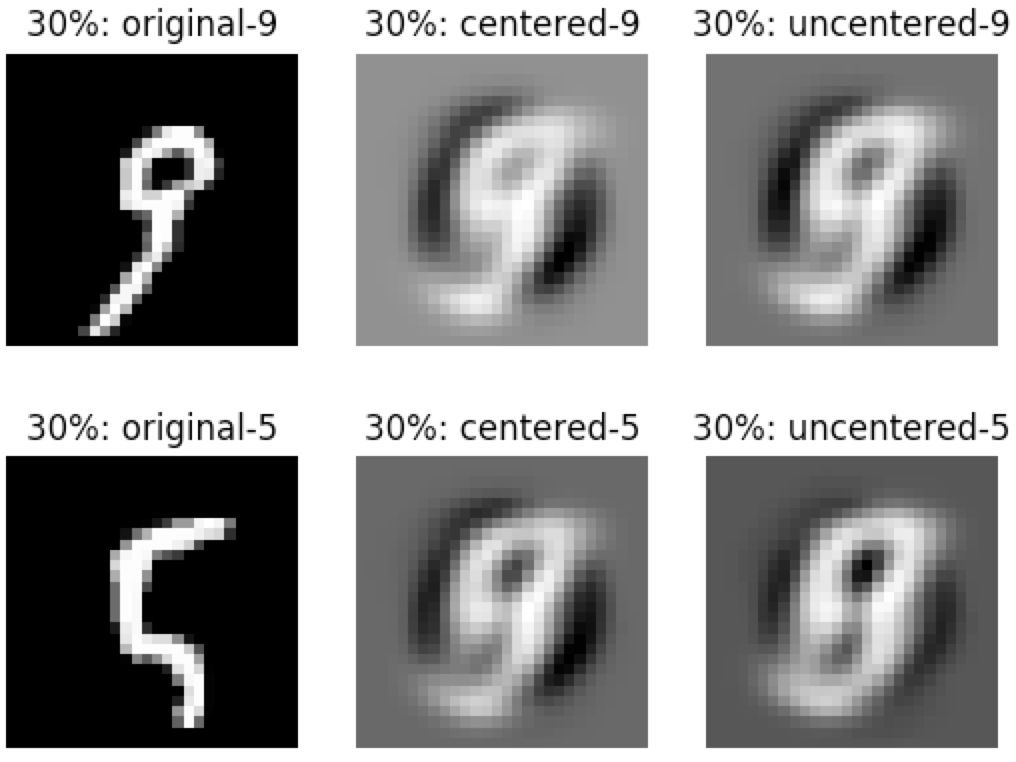
\includegraphics[scale=0.56]{30.png}
\caption{Original and reconstructed figures with 30\% information}
\end{figure}
\newpage
Preserve 60\% information:
\begin{figure}[ht]
\centering
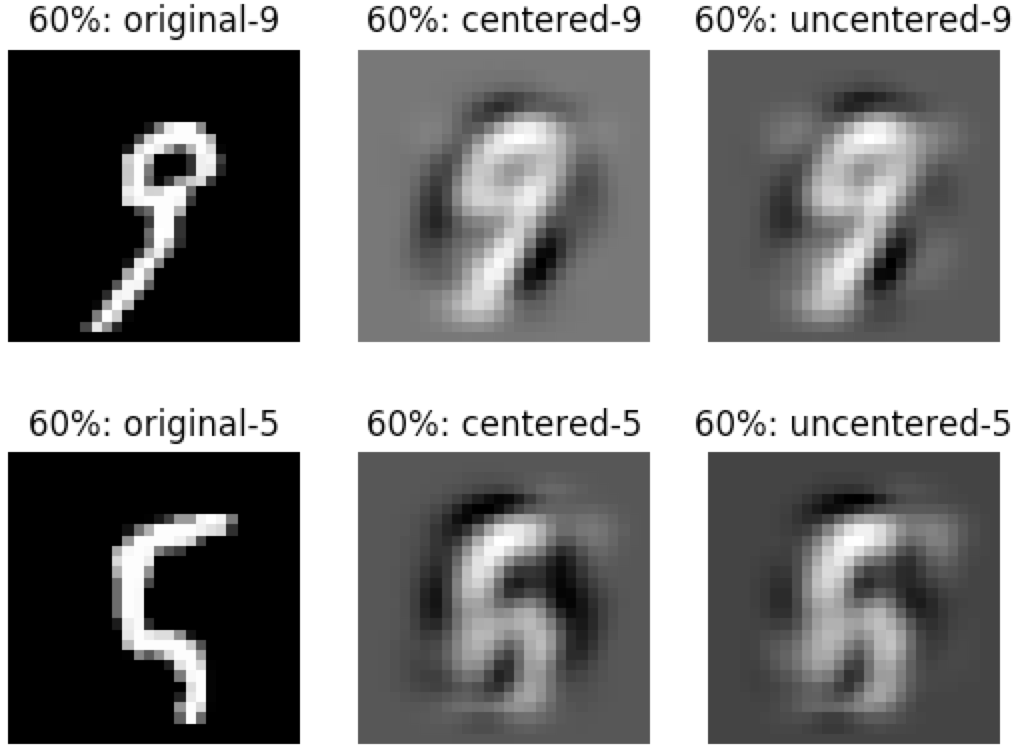
\includegraphics[scale=0.56]{60.png}
\caption{Original and reconstructed figures with 60\% information}
\end{figure}
\par
Preserve 90\% information:
\begin{figure}[ht]
\centering
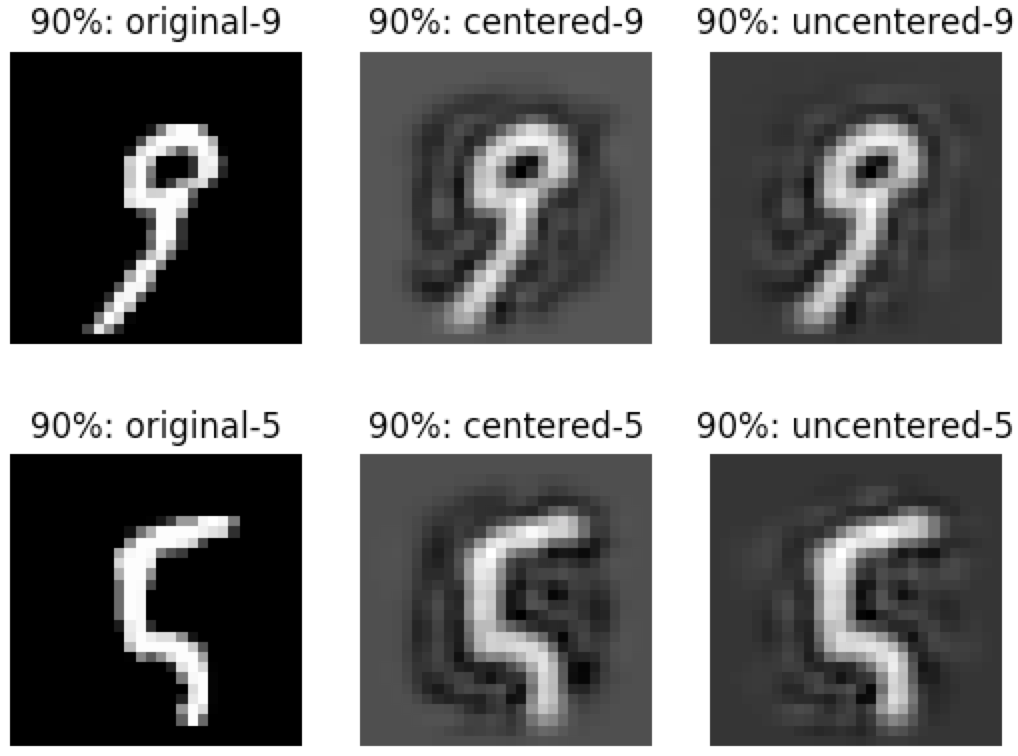
\includegraphics[scale=0.56]{90.png}
\caption{Original and reconstructed figures with 90\% information}
\end{figure}
\par
As shown in the figures, if we preserve 30\% information, the reconstructed figures can hardly be recognized. The reconstruction with 90\% information has the best performance.

\newpage
{\large \bf 2 Dimension Reduction, PCA}
\bigskip \par
{\bf 2.1 VC Dimension}
\bigskip \par
For any three dots which are not in a line, the closure of the three dots must be a triangle. If there are no positive dots, draw $H$ outside the the triangle; If there is one positive dot, draw a small $H$ to cover this dot; If there are two, with some rotation of the dots, there exists a rectangle to cover the positive dots; If there are three, draw $H$ to cover the triangle.
\par But for four dots, if there are three positive dots and one negative dot, and the negative dot locates inside the triangle of the three positive dots, then there is no rectangle to separate these dots.
\par For five dots, in the case below, the any rectangle cannot separate these dots.
\begin{figure}[ht]
\centering
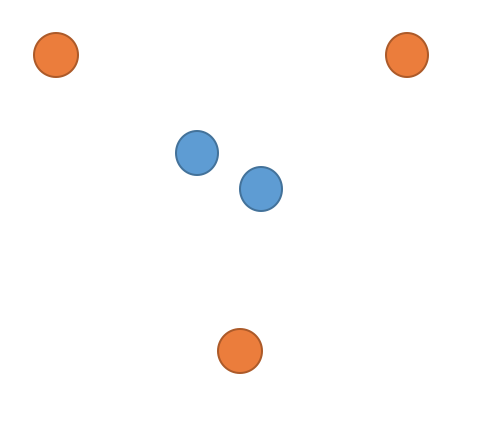
\includegraphics[scale=0.56]{5.png}
\caption{The case with 5 points that cannot be classified}
\end{figure}
\bigskip \par
{\bf 2.2 Generalization Bound}
\bigskip \par
Given the the hypothesis space $H=\{(a<x<b)|a,b\in \mathbb{R}\}$. The upper bound of the probability that a hypothesis $h\in H$ consistent with $m$ instances $x_1,\cdots,x_m$ has an error of at least $\epsilon$ is:
$$P\left(\left|R(h)-R_n(h)\right|>\epsilon\right)\leq 2\exp\left[-\frac{2m\epsilon}{(b-a)^2}\right]$$ 

\newpage
{\large \bf 3 Reinforcement Learning}
\bigskip \par
{\bf 3.1 Value Iteration}
\begin{align*}
&0.72=0+0.9\times[0.95\times(-1)+0.05\times(35)]\\
&45.695=20+0.9\times[0.2\times(-1)+0.75\times(35)+0.05\times(50)]\\
&137.71=100+0.9\times[0.1\times(-1)+0.2\times(35)+0.7\times(50)]\\
&52.71=15+0.9\times[0.1\times(-1)+0.2\times(35)+0.7\times(50)]\\
&120.68=80+0.9\times[0.05\times(-1)+0.15\times(35)+0.8\times(50)]
\end{align*}

\bigskip \par
{\bf 3.2 Policy Improvement Theorem}
\bigskip \par
Value Function: 
$$V^\pi(s)=E_\pi\{r_{t+1}+\gamma r_{t+2}+\gamma^2 r_{t+3}+\cdots|s_t=s\}=E_\pi\{r_{t+1}+\gamma V^\pi(s_{t+1})|s_t=s\}$$
State-action value function:
$$Q^\pi(s,a)=E_\pi\{r_{t+1}+\gamma V^\pi(s_{t+1})|s_t=s,a_t=a\}$$
Policy $\pi'$ is as good as or better than $\pi$ means $V^{\pi'}\geq V^\pi(s)$ for any state $s$. We need to prove $\forall s, Q^\pi\left(s,\pi'(s)\right)\geq V^\pi(s)\Rightarrow V^{\pi'}(s)\geq V^\pi(s)$:
\begin{align*}
V^\pi(s)&\leq Q^\pi(s,\pi'(s))\\
&=E_{\pi'}\{r_{t+1}+\gamma V^\pi(s_{t+1})|s_t=s\}\\
&\leq E_{\pi'}\{r_{t+1}+\gamma Q^\pi(s_{t+1},\pi'(s_{t+1}))|s_t=s\}\\
&= E_{\pi'}\{r_{t+1}+\gamma r_{t+2}+\gamma^2V^\pi(s_{t+2})|s_t=s\}\\
&\leq E_{\pi'}\{r_{t+1}+\gamma r_{t+2}+\gamma^2 r_{t+3}+\gamma^3V^\pi(s_{t+3})|s_t=s\}\\
&\;\;\vdots\\
&\leq E_{\pi'}\{r_{t+1}+\gamma r_{t+2}+\gamma^2 r_{t+3}+\gamma^3 r_{t+4} + \cdots|s_t=s\}\\
&=V^{\pi'}(s)
\end{align*}
Use a greedy way as the policy improvement strategy:
$$\pi'(s)=\mathop{\arg\max}_aQ^\pi(s,a)=\mathop{\arg\max}_aE_\pi\{r_{t+1}+\gamma V^\pi(s_{t+1})|s_t=s,a_t=a\}$$
Then we can get a new policy that is as good as or better than the old policy.
\par
If $\pi'(s)$ is as good as but not better than $\pi(s)$, then $V^{\pi'}(s)=V^{\pi}(s)$. At this time there is:
$$V^{\pi'}(s)=\max_aE_\pi\{r_{t+1}+\gamma V^\pi(s_{t+1})|s_t=s,a_t=a\}$$
which equals to the formula of optimal value function in the slide 18.
\par Thus in PI, either $\pi'$ is strictly better than $\pi$ , or $\pi$ is optimal.

\bigskip \par
{\bf 3.3 TianShou}
\bigskip \par
DQN is an off-policy, value-based algorithm.
\par
\end{document}